% SPDX-License-Identifier: CC-BY-NC-SA-4.0
%
% 07-under-pressure.tex -- wouldn't want to mess up the brakes
% Copyright (C) 2024  Jacob Koziej <jacobkoziej@gmail.com>

\documentclass{article}

% SPDX-License-Identifier: CC-BY-NC-SA-4.0
%
% preamble.tex -- document configuration
% Copyright (C) 2024  Jacob Koziej <jacobkoziej@gmail.com>

\usepackage{geometry}
\geometry{
	marginpar=1.8cm,
	paper=b5paper,
}

\usepackage{bookmark}
\usepackage{fancyhdr}
\usepackage{fontawesome}
\usepackage{marginnote}
\usepackage{titling}

\usepackage{mathtools}
\usepackage{unicode-math}
\unimathsetup{
	math-style=ISO,
	warnings-off={
		mathtools-colon,
		mathtools-overbracket,
	},
}

\usepackage{minted}
\setminted{
	breaklines,
	linenos,
	obeytabs,
}

\input{git-hash}

\author{Jacob~Koziej}

\pagestyle{fancy}
\setcounter{secnumdepth}{0}

\fancyhead{}
\fancyhead[L]{%
	\small\slshape%
	ECE 210: MATLAB Seminar -- Signals \& Systems%
}
\fancyhead[R]{%
	\scriptsize\ttfamily%
	\faCodeFork\,\gitHash\gitDirty%
}
\fancyfoot{}
\fancyfoot[L]{%
	\scriptsize\slshape%
	Copyright \copyright\ 2024 \theauthor%
	~---~%
	\ttfamily%
	\href{https://creativecommons.org/licenses/by-nc-sa/4.0/}%
	{CC BY-NC-SA 4.0}%
}
\fancyfoot[R]{%
	\scriptsize\ttfamily%
	\href{https://github.com/jacobkoziej/jk-ece210}%
	{github.com/jacobkoziej/jk-ece210}%
}
\RenewDocumentCommand{\footrule}{}{\rule{\headwidth}{\headrulewidth}}
\RenewDocumentCommand{\footruleskip}{}{1pt}

\NewDocumentCommand{\aside}{m}{%
	\marginnote{%
		\footnotesize%
		\raggedright%
		\textsl{\textbf{Aside---}}%
		\par\noindent%
		#1%
	}
}

\NewDocumentCommand{\footurl}{m}{\footnote{\url{#1}}}

\NewDocumentCommand{\mCommand}{om}{%
	\IfValueTF{#1} {%
		\href{#1}{\mintinline{matlab}{#2}}%
	} {%
		\mintinline{matlab}{#2}%
	}%
}

\NewDocumentCommand{\matrixField}{mmm}{%
	\symrm{M}_{#1 \times #2} (\symbb{#3})%
}

\NewDocumentCommand{\renderTitle}{}{%
	{\noindent\LARGE\scshape\thetitle\vspace{1ex}}%
	\pdfbookmark[1]{\thetitle}{title}%
}

\NewDocumentCommand{\vocab}{m}{\textsl{\textbf{#1}}}

\title{Assignment 07: Under Pressure}
% SPDX-License-Identifier: CC-BY-NC-SA-4.0
%
% postamble.tex -- document configuration, continued...
% Copyright (C) 2024  Jacob Koziej <jacobkoziej@gmail.com>

\usepackage{hyperref}
\hypersetup{
	hidelinks,
	pdfinfo = {
		Title    = \thetitle,
		Author   = \theauthor,
		Subject  = MATLAB,
		Keywords = {MATLAB, programming},
	},
}


\begin{document}
\renderTitle

Now that we've learned how to design filters, how about we apply what
we've learned to do some real DSP?

At Autonomy Lab, we recently redesigned our EV's braking system to pull
on the brake pedal using feedback from a pressure sensor attached to the
brake line.  The signal from the pressure sensor feeds into one of the
built-in \vocab{analog-to-digial converters (ADCs)} of an ESP32-S3
microcontroller where a brake control loop runs.  The issue with this
setup is that the signal from this sensor has a lot of noise, and to add
insult to injury, the ADC found on the ESP32-S3 is of poor quality; all
of this results in a feedback signal that is useless for PID control.

When designing this system, we gathered preliminary ADC data to see if
we could even salvage the signal.  Here are some things to note about
the data you'll be working with:

\begin{itemize}
	\item
		We sampled at 80~kHz with no hardware low-pass filter to
		determine how much we can lower the sample rate.
		\aside{Typically, you'd add a hardware low-pass filter
		to the input of an ADC at the Nyquist frequency to
		mitigate aliasing, but you'll see that we can get away
		without this!}

	\item
		The input signal was between 0 and 3.3~V and quantized
		to 12 bits by the ADC.  Note that for this test, we
		hadn't yet removed the inherent DC bias of the pressure
		sensor nor amplified the sensor's signal to utilize the
		full range of the ADC.

	\item
		We pressurized the brake line using a Hydrastar trailer
		brake at 40\% power for 1000~ms after a delay of 10~ms.

	\item
		You can find the CSV with the data here: \url{https://%
		raw.githubusercontent.com/jacobkoziej/jk-ece210/master/%
		src/assignments/07-under-pressure.d/40p_1000ms.csv}
\end{itemize}

\begin{enumerate}[leftmargin=*]
	\item
		Use \mCommand[https://www.mathworks.com/help/matlab/%
		ref/readmatrix.html]{readmatrix()} to read the CSV.  The
		first column enumerates the samples, and the second
		column contains the quantized ADC sample. \aside{Since
		this is running on a microcontroller with strict timing
		requirements, we make the transition band larger than
		desired to decrease the filter order and as a result,
		the CPU time spent filtering.}

	\item
		Normalize the signal between 0 and 1, take the DFT, and
		remove the negative frequencies since this a real
		signal.  Next, plot the DFT on a dB scale between 5 and
		40~Hz.  Add a title and axis labels, and use \mCommand[%
		https://www.mathworks.com/help/matlab/ref/yline.html]{%
		yline()} to add dashed lines at -20 and -40~dB from the
		peak frequency on the plot.

	\item
		Using the -20~dB dashed line on the previous plot,
		determine the corner frequency for an elliptic low-pass
		filter.  Have at most 0.1~dB of passband ripple,
		attenuate by 40~dB in the stopband, and allow for a
		10~Hz transition band.

	\item
		Obtain a SOS digital filter and plot its magnitude
		response on the dB scale up to \(f\)\textsubscript{stop%
		}~+~20~Hz.  Also, add horizontal and vertical dashed
		lines to indicate the passband and stopband.

	\item
		Apply the SOS digital filter to the original signal and
		plot it alongside the original signal.  Additionally,
		add a dashed line around the DC bias for the filtered
		signal.
\end{enumerate}

If done correctly, you should achieve something similar to the
following: \aside{The initial ripple in the filtered data is due to the
jump discontinuity at \(t = 0\) and the low order of the filter.  This
isn't an issue in our application, as our brake control will operate on
the signal far beyond \(t = 0\).}

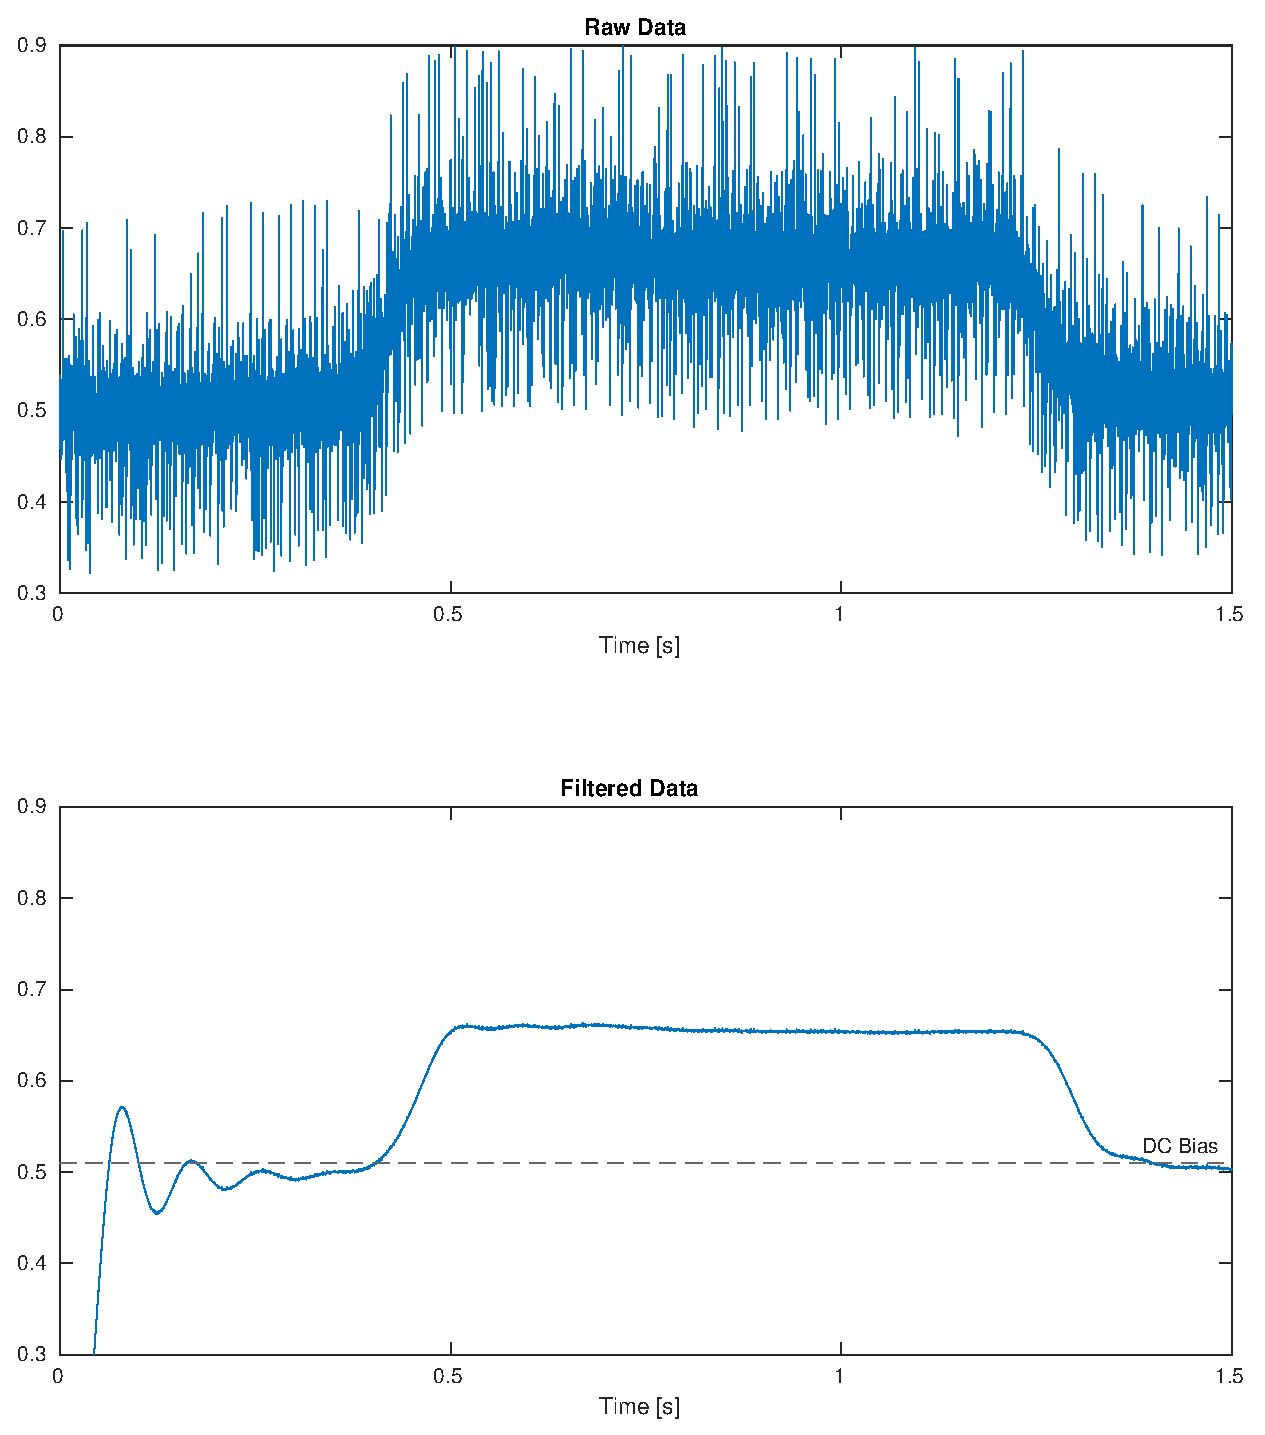
\includegraphics[width=\textwidth]{07-under-pressure.d/data.eps}
\end{document}
